\documentclass{beamer}
\usepackage{beamerthemeshadow}
\usepackage{etex}
\usepackage{tabularx}
\usepackage{booktabs}
\usepackage{layouts}
\usepackage{graphicx}
\usepackage{epstopdf}
\usepackage{amsmath}
\usepackage{eurosym}
\usetheme{Darmstadt}
\usepackage{verbatim}
\usepackage{listings}

\setbeamertemplate{navigation symbols}{}%remove navigation symbols

\newcommand{\putat}[3]{\begin{picture}(0,0)(0,0)\put(#1,#2){#3}\end{picture}}

\lstdefinestyle{customc}{
  belowcaptionskip=1\baselineskip,
  breaklines=true,
  frame=single,
  xleftmargin=\parindent,
  language=C,
  showstringspaces=false,
  basicstyle=\footnotesize\ttfamily,
  keywordstyle=\bfseries\color{green!40!black},
  commentstyle=\itshape\color{purple!40!black},
  identifierstyle=\color{blue},
  stringstyle=\color{orange},
}
\lstset{escapechar=@,style=customc}



\title[SMC and C++]{Embedding Secure Multiparty Computations\\ into C++
}

\author[Nikolaos Kofinas]{

\includegraphics[width = 2cm]{informal.pdf}\\
\textbf{Nikolaos Kofinas}\\
Department of Computer Engineering\\
University of Maryland, College Park
\vspace*{-0.8cm}
} 

\date{December 12, 2014
\vspace*{-1.2cm}
}


\setbeamertemplate{footline}[text line]{%
  \parbox{\linewidth}{\vspace*{-8pt}\insertshorttitle \hspace*{2cm} \insertshortauthor\hfill\insertframenumber}}
  
\begin{document}

\frame[plain]{\titlepage
}



\logo{
\includegraphics[height=0.6cm]{informal.pdf}}


\section[Outline]{}
\begin{frame}[fragile]
\frametitle{Presentation Outline}
\tableofcontents
\end{frame}

\section{Problem}

\section[Outline]{}
\begin{frame}[fragile]
\frametitle{Presentation Outline}
\tableofcontents[currentsection]
\end{frame}

\begin{frame}
\frametitle{What is Secure Multiparty Computations?}
\begin{itemize}
\item What it is?
\begin{figure}
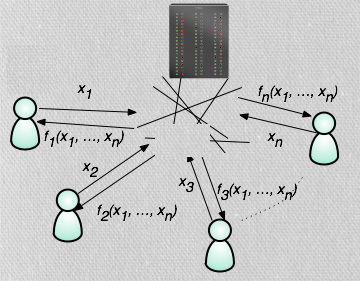
\includegraphics[width=5cm]{non_collude.png}
\caption{Source:\tiny{ \url{http://www.cs.columbia.edu/~mariana/noncollude.htm}}}
\end{figure}
\item Why we car about it?
\end{itemize}
\end{frame}


\begin{frame}
\frametitle{Related work}
\begin{itemize}
\item Languages designed for these kind of problems
\begin{itemize}
\item Wysteria
\item Fairplay
\item Ansi C
\end{itemize}
\end{itemize}
\end{frame}

\section{C++ Template Meta-programming}
\begin{frame}[fragile]
\frametitle{Presentation Outline}
\tableofcontents[currentsection]
\end{frame}

\begin{frame}[fragile]
\frametitle{C++ Templates}
\begin{itemize}
\item Generalize classes and functions
\end{itemize}

\begin{lstlisting}
template <typename T>
bool greater(T a, T b) {
    return a > b ? true : false;
}
\end{lstlisting}

\end{frame}

\begin{frame}[fragile]
\frametitle{Templates and meta-programming}
\begin{itemize}
\item Turing complete
\item Discovered by accident
\end{itemize}

\begin{lstlisting}
template <int n>
struct factorial {
	enum { value = n * factorial<n - 1>::value };
};
 
template <>
struct factorial<0> {
	enum { value = 1 };
};
...
cout << factorial<5>::value << endl;
\end{lstlisting}
\end{frame}


\begin{frame}[fragile]
\frametitle{Basics of meta-programming}
\begin{itemize}
\vspace*{-0.4cm}
\item Variables
\begin{lstlisting}
const int x = 2;
enum { y = 14 };
\end{lstlisting}
\item Functions
\begin{itemize}
\item Definition
\begin{lstlisting}
template <typename x, int y>
struct doSomething{};
\end{lstlisting}
\item Implementation and specializations
\begin{lstlisting}
template <int y>
struct doSomething<int>{
    static const int result = y*2;
};
template <int y>
struct doSomething<float>{
    static const int result = y*202;
};
\end{lstlisting}
\end{itemize}
\end{itemize}


\end{frame}

\section{Our approach}
\begin{frame}[fragile]
\frametitle{Presentation Outline}
\tableofcontents[currentsection]
\end{frame}

\begin{frame}[fragile]
\frametitle{What was the plan?}
\begin{itemize}
\item What we needed?
\begin{itemize}
\item Needed compile time verification of the user code
\end{itemize}
\item How can we do that?
\begin{itemize}
\item Create a Domain Specific Language
\end{itemize}
\item What about the boolean translation?
\begin{itemize}
\item Can be handled during run time
\end{itemize}
%\item This was the result
\end{itemize}
\end{frame}


\begin{frame}[fragile]
\frametitle{Specification of the DSL}
\begin{itemize}
\item Variables
\begin{itemize}
\item SMCvalue [bool or int]
\item sharedSMCvalue [bool or int]
\item forSMCvalue [bool or int]
\item idSMCvalue [used only to store ids]
\end{itemize}
\item Statements
\begin{itemize}
\item Plus, Minus, Logic Or...
\item Greater, Lesser, And, Or...
\item Set
\item Sequence
\item If then else
\item For
\item Return
\end{itemize}
\end{itemize}
\end{frame}

\begin{frame}[fragile]
\frametitle{Syntax of the DSL}
\begin{itemize}
\item Based on the languages that we did in class
\item It is a bit awkward for someone without template experience
\begin{lstlisting}
typedef SMCvalue<int, 1> s1;
typedef SMCvalue<int, 2> s2;
If<Greater<s1,s2>,Ret<Ip<s2> >, Ret<Id<s2> > >
\end{lstlisting}
\begin{lstlisting}
typedef SMCvalue<int, 1> s1;
typedef SMCvalue<int, 2> s2;
typedef sharedSMCvalue<int, 1> sh1;
Seq<
    Set<sh1,s1>,
    If<
        Greater<sh1,s2>,
        Ret<Id<s1> >,
        Ret<Id<s2> >
    >
>
\end{lstlisting}
\end{itemize}
\end{frame}

\begin{frame}[fragile]
\frametitle{A complete Example}
\begin{lstlisting}
typedef mySMCvalue<int, 1> s1;
typedef SMCvalue<int, 2> s2;
s1 v1;
s2 v2;
v1.value = 2;
v1.ip = myip;
v2.ip = hisip;
typedef If<
    Greater<sh1,s2>,
    Ret<Id<s1> >,
    Ret<Id<s2> >
> func;
int idOfWinner = wrapper<func>(v1,v2);
\end{lstlisting}
\end{frame}

\begin{frame}[fragile]
\frametitle{A complete Example}
\begin{lstlisting}
typedef Seq<
    Set<id1, s1>,
    Seq<
        Set<sh1, s1>,
        Seq<
            For<4, f1,
                If<Greater<f1,sh1>,
                    Seq< Set<sh1, f1>,
                        Set<id1, f1>
                    >,
                    Nope
                >
            >,
            Ret<id1>
        >
    >
>func;
int idOfWinner = wrapper<func>(v1,v2,v3,v4);
\end{lstlisting}
\end{frame}



\begin{frame}[fragile]
\frametitle{Errors}
\begin{itemize}
\item During run-time we are certain that the code is correct
\item All Errors are generated during compile time! 
\end{itemize}
\begin{lstlisting}
SMC_lang.hpp:214:9: error: static assertion failed: After Id there must be an SMVvalue!
         static_assert(!std::is_same<Expr1,Expr1>::value, "After Id there must be an SMVvalue!");
\end{lstlisting}
\end{frame}

\begin{frame}[fragile]
\frametitle{Real Error}
\begin{tiny}
\begin{lstlisting}[basicstyle=\tiny]
In file included from main.cpp:7:0:
SMC_lang.hpp: In instantiation of 'static constexpr decltype(auto) Eval<Ret<Id<Expr1> >, Env, true>::result() [with Expr1 = Greater<SMCvalue<int, 1>, SMCvalue<int, 1> >; Env = Binding<SMCvalue<int, 1>, 1, Binding<SMCvalue<int, 2>, 2, EmptyEnv> >]':
SMC_lang.hpp:135:48:   required from 'static constexpr decltype(auto) Eval<If<Cond, Then, Else>, Env, IsReturnLegal>::result() [with Cond = Greater<SMCvalue<int, 1>, SMCvalue<int, 2> >; Then = Ret<Id<Greater<SMCvalue<int, 1>, SMCvalue<int, 1> > > >; Else = Ret<Id<SMCvalue<int, 2> > >; Env = Binding<SMCvalue<int, 1>, 1, Binding<SMCvalue<int, 2>, 2, EmptyEnv> >; bool IsReturnLegal = true]'
SMC_abstract.hpp:146:43:   required from 'std::string wrapper(Args ...) [with Expr = If<Greater<SMCvalue<int, 1>, SMCvalue<int, 2> >, Ret<Id<Greater<SMCvalue<int, 1>, SMCvalue<int, 1> > > >, Ret<Id<SMCvalue<int, 2> > > >; Args = {SMCvalue<int, 1>, SMCvalue<int, 2>}; std::string = std::basic_string<char>]'
main.cpp:44:28:   required from here
SMC_lang.hpp:214:9: error: static assertion failed: After Id there must be an SMVvalue!
         static_assert(!std::is_same<Expr1,Expr1>::value, "After Id there must be an SMVvalue!");
\end{lstlisting}
\end{tiny}
\end{frame}
\section{Conclusion}

\begin{frame}[fragile]
\frametitle{Presentation Outline}
\tableofcontents[currentsection]
\end{frame}

\begin{frame}
\frametitle{Conclusion}
\begin{itemize}
\item C++ meta-programming is very strange and difficult to learn
\item You can use meta-programming for anything
\item Maybe not the best approach
\item Future work
\begin{itemize}
\item Add the boolean translation
\item Find a way to create better errors
\end{itemize}
\end{itemize}
\end{frame}

\section*{}
\begin{frame}
\frametitle{Questions}
Questions?
\end{frame}

\begin{frame}
\begin{thebibliography}{9}
\bibitem{Fairplay}Ben-David, Assaf, Noam Nisan, and Benny Pinkas. ``FairplayMP: a system for secure multi-party computation.'' Proceedings of the 15th ACM conference on Computer and communications security. ACM, 2008.
\bibitem{Ansi-c} B. Kreuter, ahbi shelat, B. Mood, and K. Butler, ``PCF: A portable
circuit format for scalable two-party secure computation.'' in USENIX,
2013
\bibitem{Wysteria}
Rastogi, Aseem, Matthew A. Hammer, and Michael Hicks. ``Wysteria: A programming language for generic, mixed-mode multiparty computations.'' (2014).
\bibitem{GMW}S. G. Choi, K.-W. Hwang, J. Katz, T. Malkin, and D. Rubenstein,
“Secure multi-party computation of boolean circuits with applications to
privacy in on-line marketplaces,” 2011, \url{http://eprint.iacr.org/}
\end{thebibliography}
\end{frame}

\begin{frame}[fragile]
\frametitle{BackUp: Implementation}
\begin{itemize}
\item We need an Environment handler
\begin{lstlisting}
template <typename Name, int Value, typename Env>
struct Binding {
    ...
} ;
typedef Binding<int, 2,
           Binding<float, 3, EmptyEnv>> Env;
           
template<typename Name, int Value, typename Env>
struct EnvLookup <Name, Binding<Name,Value,Env>> 
{  static const int res = Value;  };

template<typename Name, typename Name2,
          int Value2, typename Env>
struct EnvLookup<Name, Binding<Name2,Value2,Env>>{
  static const int res=EnvLookup<Name,Env>::res;
} ;
\end{lstlisting}
\end{itemize}
\end{frame}

\begin{frame}[fragile]
\frametitle{BackUp: Implementation}
\begin{itemize}
\item We followed the left side first eval approach
\begin{lstlisting}
template <typename Exp, typename Env, bool IsReturnLegal>
struct Eval {} ;

template <typename Expr1, typename Expr2>
struct Plus {} ;

template <typename Expr1, typename Expr2,
         typename Env, bool IsReturnLegal>
struct Eval<Plus<Expr1,Expr2>, Env, IsReturnLegal>
{
...
};
\end{lstlisting}
\end{itemize}
\end{frame}
\end{document}
